% Individual deliverables (D1--D5). Included from lab9_report.tex.
\section{Individual work}

\subsection{Deliverable 1: Spy game}\label{sec:d1}

We read the block pattern of the handout spy plot cell by cell (the pattern is stored in
\code{results/d1/spy\_pattern.txt}; Fig.~\ref{fig:spy}, left, redraws it). The matrix has
20 block rows: the thick lines separate 7 past poses, the current pose and the landmarks.
We call the poses $x_1,\dots,x_8$ and the landmarks $l_1,\dots,l_{12}$. The pose--pose
block is tridiagonal (odometry links $x_i$--$x_{i+1}$), the landmark--landmark block is
diagonal, and an off-diagonal pose--landmark block is non-zero iff the pose observed the
landmark. Table~\ref{tab:spy} lists the observations.

\begin{table}[H]
\centering\footnotesize\setlength{\tabcolsep}{3.5pt}
\begin{tabular}{lcccccccc}
\toprule
pose & $x_1$ & $x_2$ & $x_3$ & $x_4$ & $x_5$ & $x_6$ & $x_7$ & $x_8$ \\
\midrule
landmarks & $l_1,l_2$ & $l_1,l_2,l_4$ & $l_1,l_2,l_4$ & $l_1,l_3,l_4,l_6$ &
$l_3,l_4,l_5,l_6$ & $l_5,l_6,l_7,l_8$ & $l_6,l_8,l_9,l_{10}$ & $l_7,l_9,l_{10},l_{11},l_{12}$ \\
count & 2 & 3 & 3 & 4 & 4 & 4 & 4 & 5 \\
\bottomrule
\end{tabular}
\caption{Pose--landmark blocks of the D1 information matrix.}\label{tab:spy}
\end{table}

\begin{enumerate}
\item \textbf{8 robot poses} (7 past poses and the current one, $x_8$).
\item \textbf{12 landmarks.}
\item The current pose $x_8$ observes \textbf{5 landmarks}: $l_7, l_9, l_{10}, l_{11}, l_{12}$.
\item \textbf{The last pose $x_8$} observes the most landmarks (5); every other pose sees 2--4.
\item The 2nd landmark $l_2$ is observed by \textbf{$x_1$, $x_2$ and $x_3$}.
\item Marginalising a variable replaces the information matrix by the Schur complement, which
  connects all of the variable's neighbours with each other. The neighbours of $l_2$ are
  $x_1,x_2,x_3$. The links $x_1$--$x_2$ and $x_2$--$x_3$ already exist, so the only fill-in
  is a new \textbf{$x_1$--$x_3$ block} (and its transpose); row and column $l_2$ disappear and
  everything else stays the same (Fig.~\ref{fig:spy}, middle, fill-in in red).
\item The past poses $x_1,\dots,x_7$ form a connected chain, so eliminating all of them
  makes their whole Markov blanket a clique. The blanket is $x_8$ (odometry link from $x_7$)
  and every landmark that a past pose has seen, $l_1,\dots,l_{10}$. The result is a
  \textbf{fully dense $11\times11$ block over $\{x_8,l_1,\dots,l_{10}\}$}. Only $l_{11}$ and
  $l_{12}$, which only the current pose saw, keep their sparse rows (diagonal block plus the
  link to $x_8$) (Fig.~\ref{fig:spy}, right). This is why filtering approaches (EKF-SLAM,
  which keep only the current pose) end up with a dense covariance/information matrix.
\item A variable can be marginalised without fill-in iff its neighbours are already pairwise
  connected. In this matrix that holds for the landmarks seen by a single pose or by two
  consecutive poses: \textbf{$l_{11}$, $l_{12}$} (seen only by $x_8$), and also $l_3$ ($x_4,x_5$),
  $l_5$ ($x_5,x_6$), $l_8$ ($x_6,x_7$), $l_9$ and $l_{10}$ ($x_7,x_8$). Marginalising any pose
  creates fill-in, because a pose links its landmarks with each other and with the
  neighbouring poses, and those links do not exist yet (landmarks are never directly
  connected). We checked every case with a symbolic elimination in
  \code{scripts/make\_figures.py}.
\item Both images show the pose--pose block after eliminating all landmarks: poses $i$ and
  $j$ are linked iff they observed a common landmark.
  \begin{itemize}
  \item \textbf{Left (100 poses, density 0.40):} almost every pose shares landmarks with
    almost every other pose, including poses far apart in time. The robot kept seeing the
    same small set of landmarks for the whole run, so it was \emph{surveying a small
    area} (e.g.\ a single room, or moving back and forth/looping inside it). The reduced
    camera system is nearly dense, so solving it costs close to $O(n^3)$.
  \item \textbf{Right (about 850 poses, density 0.014):} the matrix is banded, so each
    pose only shares landmarks with poses close to it in time. The robot was
    \emph{exploring a large environment} (e.g.\ a long corridor or a large building) and
    rarely came back. The few off-diagonal segments are \emph{revisits/loop closures}: around
    poses 270--350 the robot saw again the place it saw around poses 500--570 (the
    segment runs parallel to the diagonal, so it went through it in the same direction),
    and the short blocks near poses 0/630, 650/820 and 730/810 are brief revisits.
    The thicker blocks around poses 650--700 and 720--740 mean that the robot moved slowly or
    rotated in place there, so many consecutive poses saw the same landmarks.
  \end{itemize}
\end{enumerate}

\begin{figure}[H]
\centering
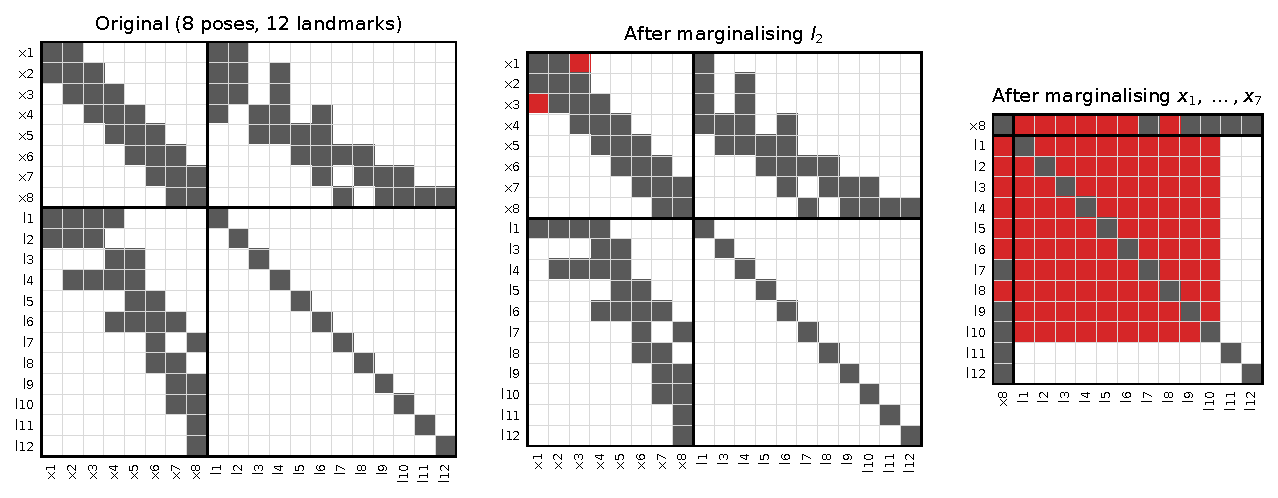
\includegraphics[width=\linewidth]{d1_spy_marginalization.pdf}
\caption{D1: block pattern of the handout matrix (left; poses $x$, landmarks $l$) and the
predicted pattern after marginalising $l_2$ (middle, question 6) and after marginalising
all past poses (right, question 7). Red blocks are fill-in created by the Schur complement.}
\label{fig:spy}
\end{figure}

\subsection{Deliverable 2: Well-begun is half done}\label{sec:d2}

\textbf{Proposal:} fix the root pose to the identity, compute a \emph{shortest-path
spanning tree} of the pose graph from the root (breadth-first search when all edges are
equally accurate; Dijkstra with edge weights equal to the measurement uncertainty, e.g.\
the trace of each edge's covariance, when they are not), and initialise every node by
composing the relative measurements along its tree path from the root.

\textbf{Rationale:} the initialisation error of a node grows with the number (and
uncertainty) of the measurements chained to reach it. Odometric chaining uses the path
$0\to1\to\dots\to i$, of length $i$. The shortest path also uses loop closures as
shortcuts, so on a graph with loops the hop count drops from $O(N)$ to the graph diameter,
and the accumulated noise drops with it. The method needs no special graph topology and
costs only $O(|\mathcal{E}|\log|\mathcal{V}|)$.

\subsection{Deliverable 3: Feature-based methods for SLAM (ORB-SLAM)}\label{sec:d3}

\paragraph{1. Modules (Fig.~1 of~\cite{murartal2015orb}).}
\begin{itemize}
\item \textbf{Map}: map points (3D position, viewing direction, representative ORB
  descriptor, scale-invariance range) and keyframes (pose, intrinsics, ORB features); the
  keyframes are connected by three graphs: the \emph{covisibility graph} (an edge when two
  keyframes share at least 15 map points), the \emph{spanning tree} and the sparse
  \emph{essential graph} (spanning tree, strong covisibility edges with at least 100
  shared points, and loop-closure edges).
\item \textbf{Place recognition}: a DBoW2 bag-of-words \emph{recognition database} of
  keyframes, built on an offline ORB \emph{visual vocabulary}; it is queried for
  relocalisation and for loop detection.
\item \textbf{Map initialisation}: computes a homography and a fundamental matrix in parallel
  from the first two frames, chooses one of them with a heuristic score, and builds the
  initial map by triangulation followed by full bundle adjustment.
\item \textbf{Tracking} (thread): extracts ORB features in every frame, estimates the
  camera pose from the previous frame with a constant-velocity model (or by global
  relocalisation when tracking is lost), refines it against the \emph{local map} (keyframes
  covisible with the current one) with motion-only BA, and decides whether to insert a new
  keyframe.
\item \textbf{Local mapping} (thread): processes new keyframes; it updates the covisibility
  graph, culls map points that are rarely found, triangulates new points from matches with
  covisible keyframes, runs \emph{local BA} on the current keyframe, its covisible keyframes
  and their points, and culls redundant keyframes (90\,\% of their points seen in at least
  three other keyframes).
\item \textbf{Loop closing} (thread): for each new keyframe, detects loop candidates with
  the bag-of-words database, computes the similarity transform $\mathrm{Sim}(3)$ to the loop
  keyframe (which also corrects scale drift), fuses the duplicated map points and
  corrects the poses on both sides of the loop, and finally optimises the \emph{essential
  graph} in $\mathrm{Sim}(3)$ to spread the loop correction over the whole map.
\end{itemize}

\paragraph{2. Wrong loop closures.}
ORB-SLAM accepts a loop only after several checks.
(i) \emph{Appearance}: a candidate keyframe must have a bag-of-words similarity higher than
the lowest similarity between the current keyframe and its covisible neighbours, and
keyframes already connected to the current one are excluded.
(ii) \emph{Temporal consistency}: a candidate is accepted only if three consecutive
keyframes produce loop candidates that are consistent, i.e.\ connected in the covisibility
graph.
(iii) \emph{Geometric verification}: ORB correspondences with the candidate are fed to
RANSAC with a $\mathrm{Sim}(3)$ solver (Horn's method); the transform is then refined, more
correspondences are searched with guided matching and the transform is optimised again. The
loop is accepted only with enough inliers (at least 40).

If a wrong loop passes these checks anyway, the method has no back-end mechanism to reject
it. The loop fusion merges map points that are actually different, and essential-graph
optimisation (a plain least-squares problem without robust kernels on the loop edges) pulls
the two places together. This bends and distorts the trajectory and the map
\emph{globally}. Later tracking and local BA are then done against a corrupted map, which
leads to more bad data associations and often to tracking failure. The error is not
undone later. This is why the checks above are very strict: ORB-SLAM gives up recall to
get near-perfect precision. Later systems added robust back-ends against outlier loops,
e.g.\ switchable constraints or pairwise consistency maximisation in Kimera-RPGO.

\subsection{Deliverable 4 (optional): Direct methods for SLAM (LSD-SLAM)}\label{sec:d4}

\paragraph{1. Modules of LSD-SLAM~\cite{engel2014lsd}.}
\begin{itemize}
\item \textbf{Tracking}: estimates the $\mathrm{SE}(3)$ pose of each new frame with respect to
  the current keyframe by minimising the variance-normalised photometric error over the
  pixels with depth (direct image alignment, Gauss--Newton on a pyramid).
\item \textbf{Depth map estimation}: refines the semi-dense inverse-depth map of the current
  keyframe with small-baseline stereo comparisons and filtering of tracked frames; when
  the camera moves too far, it creates a new keyframe by propagating the depth map to it.
\item \textbf{Map optimisation}: keyframes are added to a pose graph of $\mathrm{Sim}(3)$
  constraints, which come from direct $\mathrm{Sim}(3)$ image alignment between keyframes
  (with a depth residual, so scale drift is observable); the graph is optimised
  continuously in the background (g2o), and loop closures are found with FAB-MAP plus
  nearby keyframes.
\end{itemize}
\textbf{Similarities with ORB-SLAM:} keyframe-based design, separate tracking and mapping
threads, monocular input, $\mathrm{Sim}(3)$ pose graph to handle scale drift, appearance-based
loop detection with geometric verification. \textbf{Differences:} LSD-SLAM uses raw intensities
(photometric error) instead of ORB keypoints and reprojection error; it builds a
\emph{semi-dense} depth map (all pixels with enough gradient) instead of a sparse point map;
its back-end is a keyframe pose graph without bundle adjustment over the structure; and it
uses no descriptors, so its relocalisation is weaker.

\paragraph{2. Robustness.}
Feature-based methods are more robust to illumination changes and occlusions. Direct methods
assume brightness constancy: a change in exposure, auto-gain or lighting changes $I(p)$ and
biases the photometric error directly, unless one models affine brightness and calibrates
the camera photometrically as DSO does. Descriptors such as ORB/BRIEF use intensity
comparisons, which are invariant to monotonic brightness changes. Occluded points also simply fail to
match and are rejected by RANSAC or by robust kernels. In a direct method they become large
photometric residuals that enter a dense, non-convex alignment with a small convergence
basin. Direct methods are better in low-texture scenes and with motion blur, where keypoints
are scarce.

\subsection{Deliverable 5 (optional): From landmark-based SLAM to rotation estimation}\label{sec:d5}

\paragraph{Elimination of translations and landmarks.}
Since the Euclidean norm is invariant to rotations, $\|R_i^\top v\|=\|v\|$, so the first two
terms of problem~(1) are equal to
\begin{equation}
\sum_{(i,k)\in\mathcal{E}_l}\|p_k-t_i-R_i\bar p_{ik}\|_2^2
+\sum_{(i,j)\in\mathcal{E}_o}\|t_j-t_i-R_i\bar t_{ij}\|_2^2 .
\end{equation}
Stack the positions $x=[t_1^\top\cdots t_N^\top\ p_1^\top\cdots p_M^\top]^\top\in\mathbb{R}^{3(N+M)}$
and consider the graph whose nodes are poses and landmarks and whose $E=|\mathcal{E}_l|+|\mathcal{E}_o|$
edges are the observation and odometry edges. Let $A\in\mathbb{R}^{E\times(N+M)}$ be its
incidence matrix (row $e=(a,b)$ has $-1$ in column $a$ and $+1$ in column $b$) and
$\bar A=A\otimes I_3$. Each measured vector enters as $R_i\bar m_e$ with $\bar m_e\in\{\bar p_{ik},\bar t_{ij}\}$,
and $R_i\bar m_e=(\bar m_e^\top\otimes I_3)\,\mathrm{vec}(R_i)$ is linear in the rotations.
With $r=[\mathrm{vec}(R_1)^\top\cdots\mathrm{vec}(R_N)^\top]^\top\in\mathbb{R}^{9N}$ there is a
constant sparse matrix $B\in\mathbb{R}^{3E\times 9N}$ (row block $e$ has
$\bar m_e^\top\otimes I_3$ in the column block of the observing pose $i$) such that the
stacked measurements are $Br$. Problem~(1) becomes
\begin{equation}
\min_{R_i\in\mathrm{SO}(3)}\ \min_{x}\ \|\bar A x - Br\|_2^2 + \sum_{(i,j)\in\mathcal{E}_o}\|R_j-R_i\bar R_{ij}\|_F^2 .
\end{equation}
For fixed rotations the inner problem is an unconstrained \emph{linear} least-squares
problem in $x$ (the rotation term does not depend on $x$). Fixing the gauge ($t_1=0$, i.e.\
removing the first column block of $\bar A$, which leaves $\bar A$ with full column rank if
the graph is connected), its minimiser is
$x^\star(r)=(\bar A^\top\bar A)^{-1}\bar A^\top B r$, and the minimum value is
$\|(I-\bar A(\bar A^\top\bar A)^{-1}\bar A^\top)Br\|^2=r^\top B^\top \Pi B r$, where
$\Pi=I-\bar A(\bar A^\top\bar A)^{-1}\bar A^\top$ is the orthogonal projector onto the
complement of the range of $\bar A$ (the cycle space of the graph). Substituting back, we get
the rotation-only problem
\begin{equation}
\boxed{\ \min_{R_i\in\mathrm{SO}(3),\,i=1..N}\ r^\top Q\, r+\sum_{(i,j)\in\mathcal{E}_o}\|R_j-R_i\bar R_{ij}\|_F^2,\qquad Q=B^\top\Pi B\ }
\end{equation}
which depends on the rotations only. The original optimal translations and landmarks are
recovered in closed form as $x^\star(r^\star)$. The rotation term can also be written as a
quadratic form $r^\top (L_R\otimes I_3)\,r$ with a ``connection Laplacian'' of the odometry
graph, so the whole problem is $\min_{R\in\mathrm{SO}(3)^N} r^\top \tilde Q r$, a quadratic
problem over rotations.

\paragraph{Why the smaller problem is not necessarily faster.}
Optimisation-based SLAM is fast because its Hessian/information matrix is \emph{sparse}
(each measurement only involves two variables), so sparse Cholesky with a good ordering
solves each Gauss--Newton step in about linear time. Eliminating $x$ is a Schur complement
on all positions at once. As in D1.7, it connects every pair of poses joined by a path in
the graph: $\Pi$ (and hence $Q$) is in general \emph{dense}, and $(\bar A^\top\bar A)^{-1}$ is the
inverse of a graph Laplacian, which is dense for a connected graph. The rotation problem has
$9N$ instead of $3(N+M)+9N$ unknowns, but each iteration needs a dense $O(N^2)$ matrix and
$O(N^3)$ factorisation, while the original sparse problem costs about
$O(N+M)$--$O(N^{1.5})$. Forming $Q$ itself requires factorising $\bar A^\top\bar A$. Long
trajectories have thousands of poses, so the dense rotation-only problem is slower to solve
than the larger but sparse original.
